\documentclass[tikz,border=5pt]{standalone}
\usepackage{pgfplots}
\usepgfplotslibrary{groupplots,fillbetween}

\pgfplotsset{compat=1.18}

\begin{document}
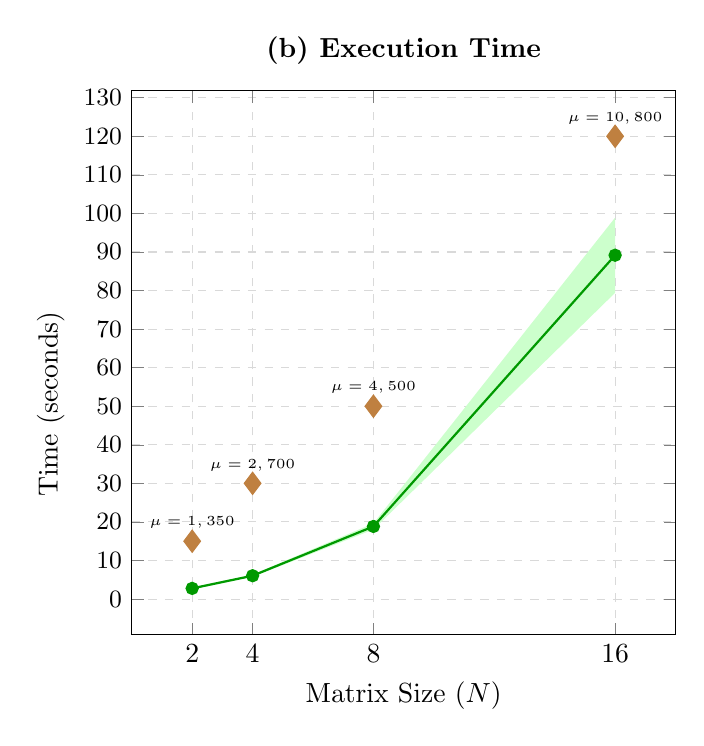
\begin{tikzpicture}
\begin{axis}[
    width=0.7\columnwidth,
    height=0.7\columnwidth,
    grid=major,
    grid style={dashed, gray!30},
    xlabel={Matrix Size ($N$)},
    xtick = {2,4,8,16},
    ylabel={Time (seconds)},
    ylabel style ={xshift=-15pt},
    title={\textbf{(b) Execution Time}},
    ytick={0,10,20,30,40,50,60,70,80,90,100,110,120,130,140},
    yticklabel style={font=\small, /pgf/number format/.cd, fixed, 1000 sep={}},
    xmin=0, xmax=18,
]
\addplot[name path=upper,draw=none] coordinates { (2, 3.0375) (4, 6.3391) (8, 19.6287) (16, 98.9039) };
\addplot[name path=lower,draw=none] coordinates { (2, 2.4996) (4, 5.7629) (8, 18.0359) (16, 79.4126) };
\addplot[green!20,area legend] fill between[of=upper and lower];
\addplot[green!60!black,thick,mark=*] coordinates { (2, 2.7685) (4, 6.0510) (8, 18.8323) (16, 89.1582) };
\addplot[brown,only marks,mark=diamond*,mark size=4pt,forget plot] coordinates { (2, 15.00) (4, 30.00) (8, 50.00) (16, 120.00) };

\node[font=\tiny, yshift=1pt] at (axis cs:2,15.00) [above] {$\mu=1,350$};
\node[font=\tiny, yshift=1pt] at (axis cs:4,30.00) [above] {$\mu=2,700$};
\node[font=\tiny, yshift=1pt] at (axis cs:8,50.00) [above] {$\mu=4,500$};
\node[font=\tiny, yshift=1pt] at (axis cs:16,120.00) [above] {$\mu=10,800$};
\end{axis}
\end{tikzpicture}
\end{document}